\begin{figure}[!h]
  \setlength{\unitlength}{\textwidth}

        \begin{picture}(1,1.1)(0,0.35)

      % % % Parkinson Data 
      \put(0.1,1.1){\includegraphics[width=0.75\unitlength]{./chapter-cross-sections/fnp/vel_prof-tri-4.eps}}
      \put(0.1,0.737){\includegraphics[width=0.75\unitlength]{./chapter-cross-sections/fnp/vel_prof-tri-16.eps}}
      \put(0.1,0.38){\includegraphics[width=0.75\unitlength]{./chapter-cross-sections/fnp/vel_prof-tri-21.eps}}
     
      
      



%      
    \put(0.21,1.41){\small(a)}
     \put(0.21,1.05){\small(b)}
     \put(0.21,0.69){\small(c)}
\put(0.1,0.95){$\displaystyle V_m$}
\put(0.1,1.3){$\displaystyle V_m$}
\put(0.1,0.56){$\displaystyle V_m$}
\put(0.34,0.35){Distance from the leading edge}

      
    \end{picture}

    \caption{Velocity magnitudes of the flow along a line parallel to the front surface spreading towards top (\dashedrule) and bottom (\solidrule) boundaries (figure \ref{fig:tri-sketch}). These two lines (for the top and bottom surfaces) start from the top and bottom leading edges of the triangular cross section. Data present (a) $\alpha=4^\circ$, (b) $\alpha=16^\circ$ \ and (c) $\alpha=21^\circ$.}
    \label{fig:vel-profile}
\end{figure}

 %vspace{10cm}
